% Licensed under the Creative Commons Attribution Share Alike 4.0 International.
% See the LICENSE file in the repository root for full license text.

\section{C++20 带来的新变化}

C++ 程序的编译速度较慢,与图 \ref{fig:build-flow} 中的预处理步骤息息相关。因为 \lstinline[language={[latest]C++}]{#include} 指令的本质是文本替换,所以处理每个源文件时都会一并处理大量头文件中的内容,导致编译速度显著降低。以 C++ 的“Hello, world!”程序为例,虽然它本身只包含下面四行代码,但编译器需要完整处理 \lstinline[language={}]{iostream} 头文件,每次编译实际上需要处理上万行代码\cite{cpp-module-1}!

\begin{lstlisting}[language={[latest]C++}, moreemph={[2]endl}]
#include <iostream>
int main()
{
	std::cout << "Hello World!" << std::endl;
}
\end{lstlisting}

C++20 标准引入了\emph{模块(module)}来解决编译速度慢的问题,引入模块后的生成流程可以用图 \ref{fig:module} 示意\cite{cpp-module-1}。从图中可以看到,引入模块后不再存在效率低下的文本替换,不会再用到 \lstinline[language={[latest]C++}]{#include} 指令。取而代之的模块接口文件只需被编译一次,就能为后续流程提供可以快速读取的接口信息缓存。实践表明,使用模块可以得到十倍量级的编译性能提升\cite{cpp-module-2}。

\begin{figure}[H]
	\centering
	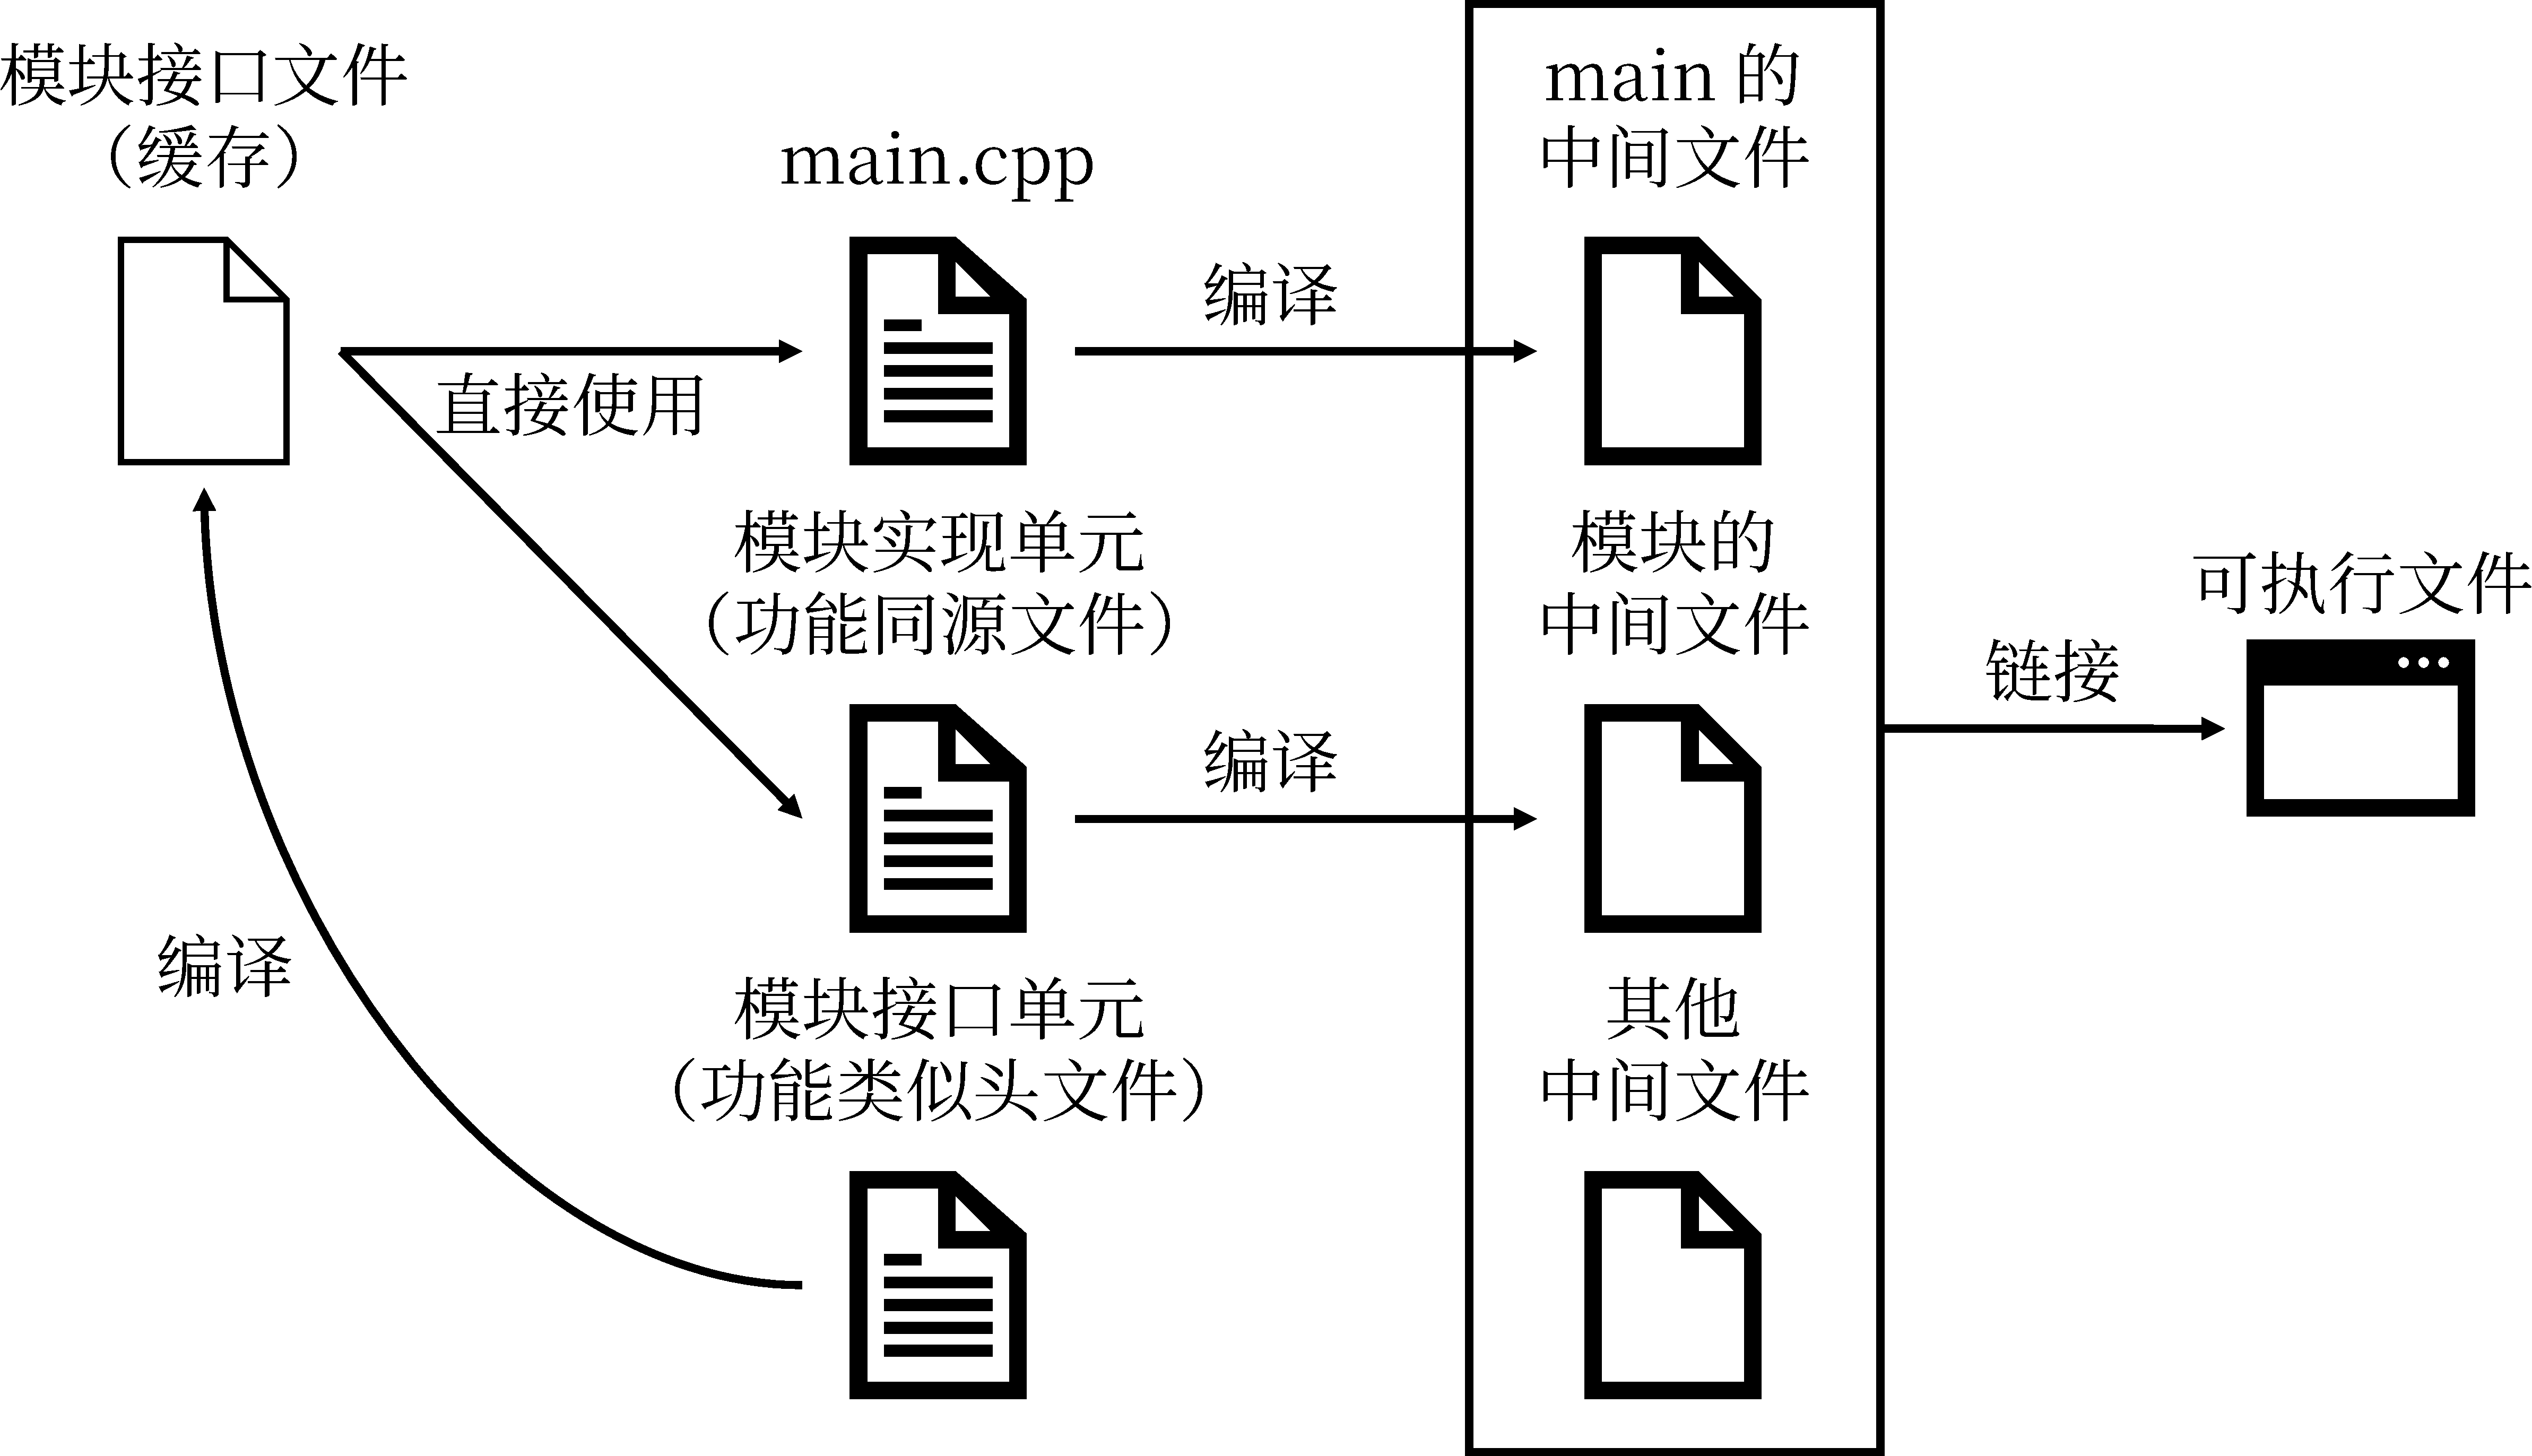
\includegraphics[scale=0.15]{assets/module}
	\caption{使用模块的生成流程示意图。}
	\label{fig:module}
\end{figure}

模块还可以增强代码之间的隔离性,可以指定模块内部导入的其他模块无法被外部使用\cite{cpp-module-3}。尽管模块具有上述优点,但目前仍然没有完全支持该特性的编译器和 IDE,即将开始学习的 CMake 也尚不支持模块的处理。模块作为一个现代的全新特性,我们可以期待它在未来彻底代替 C++ 传统的 \lstinline[language={[latest]C++}]{#include} 指令,但可能需要数年乃至数十年的时间。